\section{Постановка задачи}

Требуется реализовать обход препятствия (клетка с координатами (4, 6)) на карте, полученной в лабораторной работе №1, с помощью изменения весов контрольных точек B-сплайна. Необходимо обеспечить плавное отклонение траектории от исходного пути при сохранении характеристик B-сплайна.

\section{Теоретические основы}

B-сплайны являются эффективным инструментом для сглаживания дискретных траекторий, обеспечивая локальный контроль формы кривой через контрольные точки. Применение весов позволяет модифицировать влияние каждой контрольной точки на результирующую траекторию.

Функционал минимизации для сглаженного B-сплайна имеет вид:

$$\min \sum_{i=1}^{n} w_i (y_i - f(x_i))^2 + s \int (f''(x))^2 dx$$

где:
\begin{itemize}
\item $w_i$ --- веса контрольных точек
\item $s$ --- параметр сглаживания
\item $f(x)$ --- результирующая сглаженная функция
\end{itemize}

Применение весов в данной задаче основано на принципе "ослабления" влияния точек, находящихся рядом с препятствием. Уменьшение весов точек, близких к целевой клетке, позволяет траектории B-сплайна "пролететь мимо" препятствия, плавно обходя его.

\section{Методика обхода препятствия}

Для обхода клетки (4, 6) применяется следующая стратегия:
\begin{enumerate}
\item Загружаются карта и путь A*, построенные в лабораторной работе №1
\item Вычисляется расстояние от каждой точки пути до целевой клетки
\item Точки, близкие к препятствию, получают уменьшенные веса (0.3)
\item Точки, удаленные от препятствия, получают нормальные веса (1.0)
\item Точки, значительно удаленные от препятствия, получают повышенные веса (0.5) для усиления их влияния
\item Применяется параметр сглаживания $s = 0.5$ для сохранения плавности траектории
\end{enumerate}

\section{Результаты}

На рисунке \ref{fig:weighted_bspline} представлена B-сплайн траектория с обходом клетки (4, 6). Оранжевые звездочки обозначают точки с повышенными весами (для усиления влияния), циановые --- точки с уменьшенными весами (вблизи препятствия), белые --- точки с нормальными весами.

\begin{figure}[H]
\centering
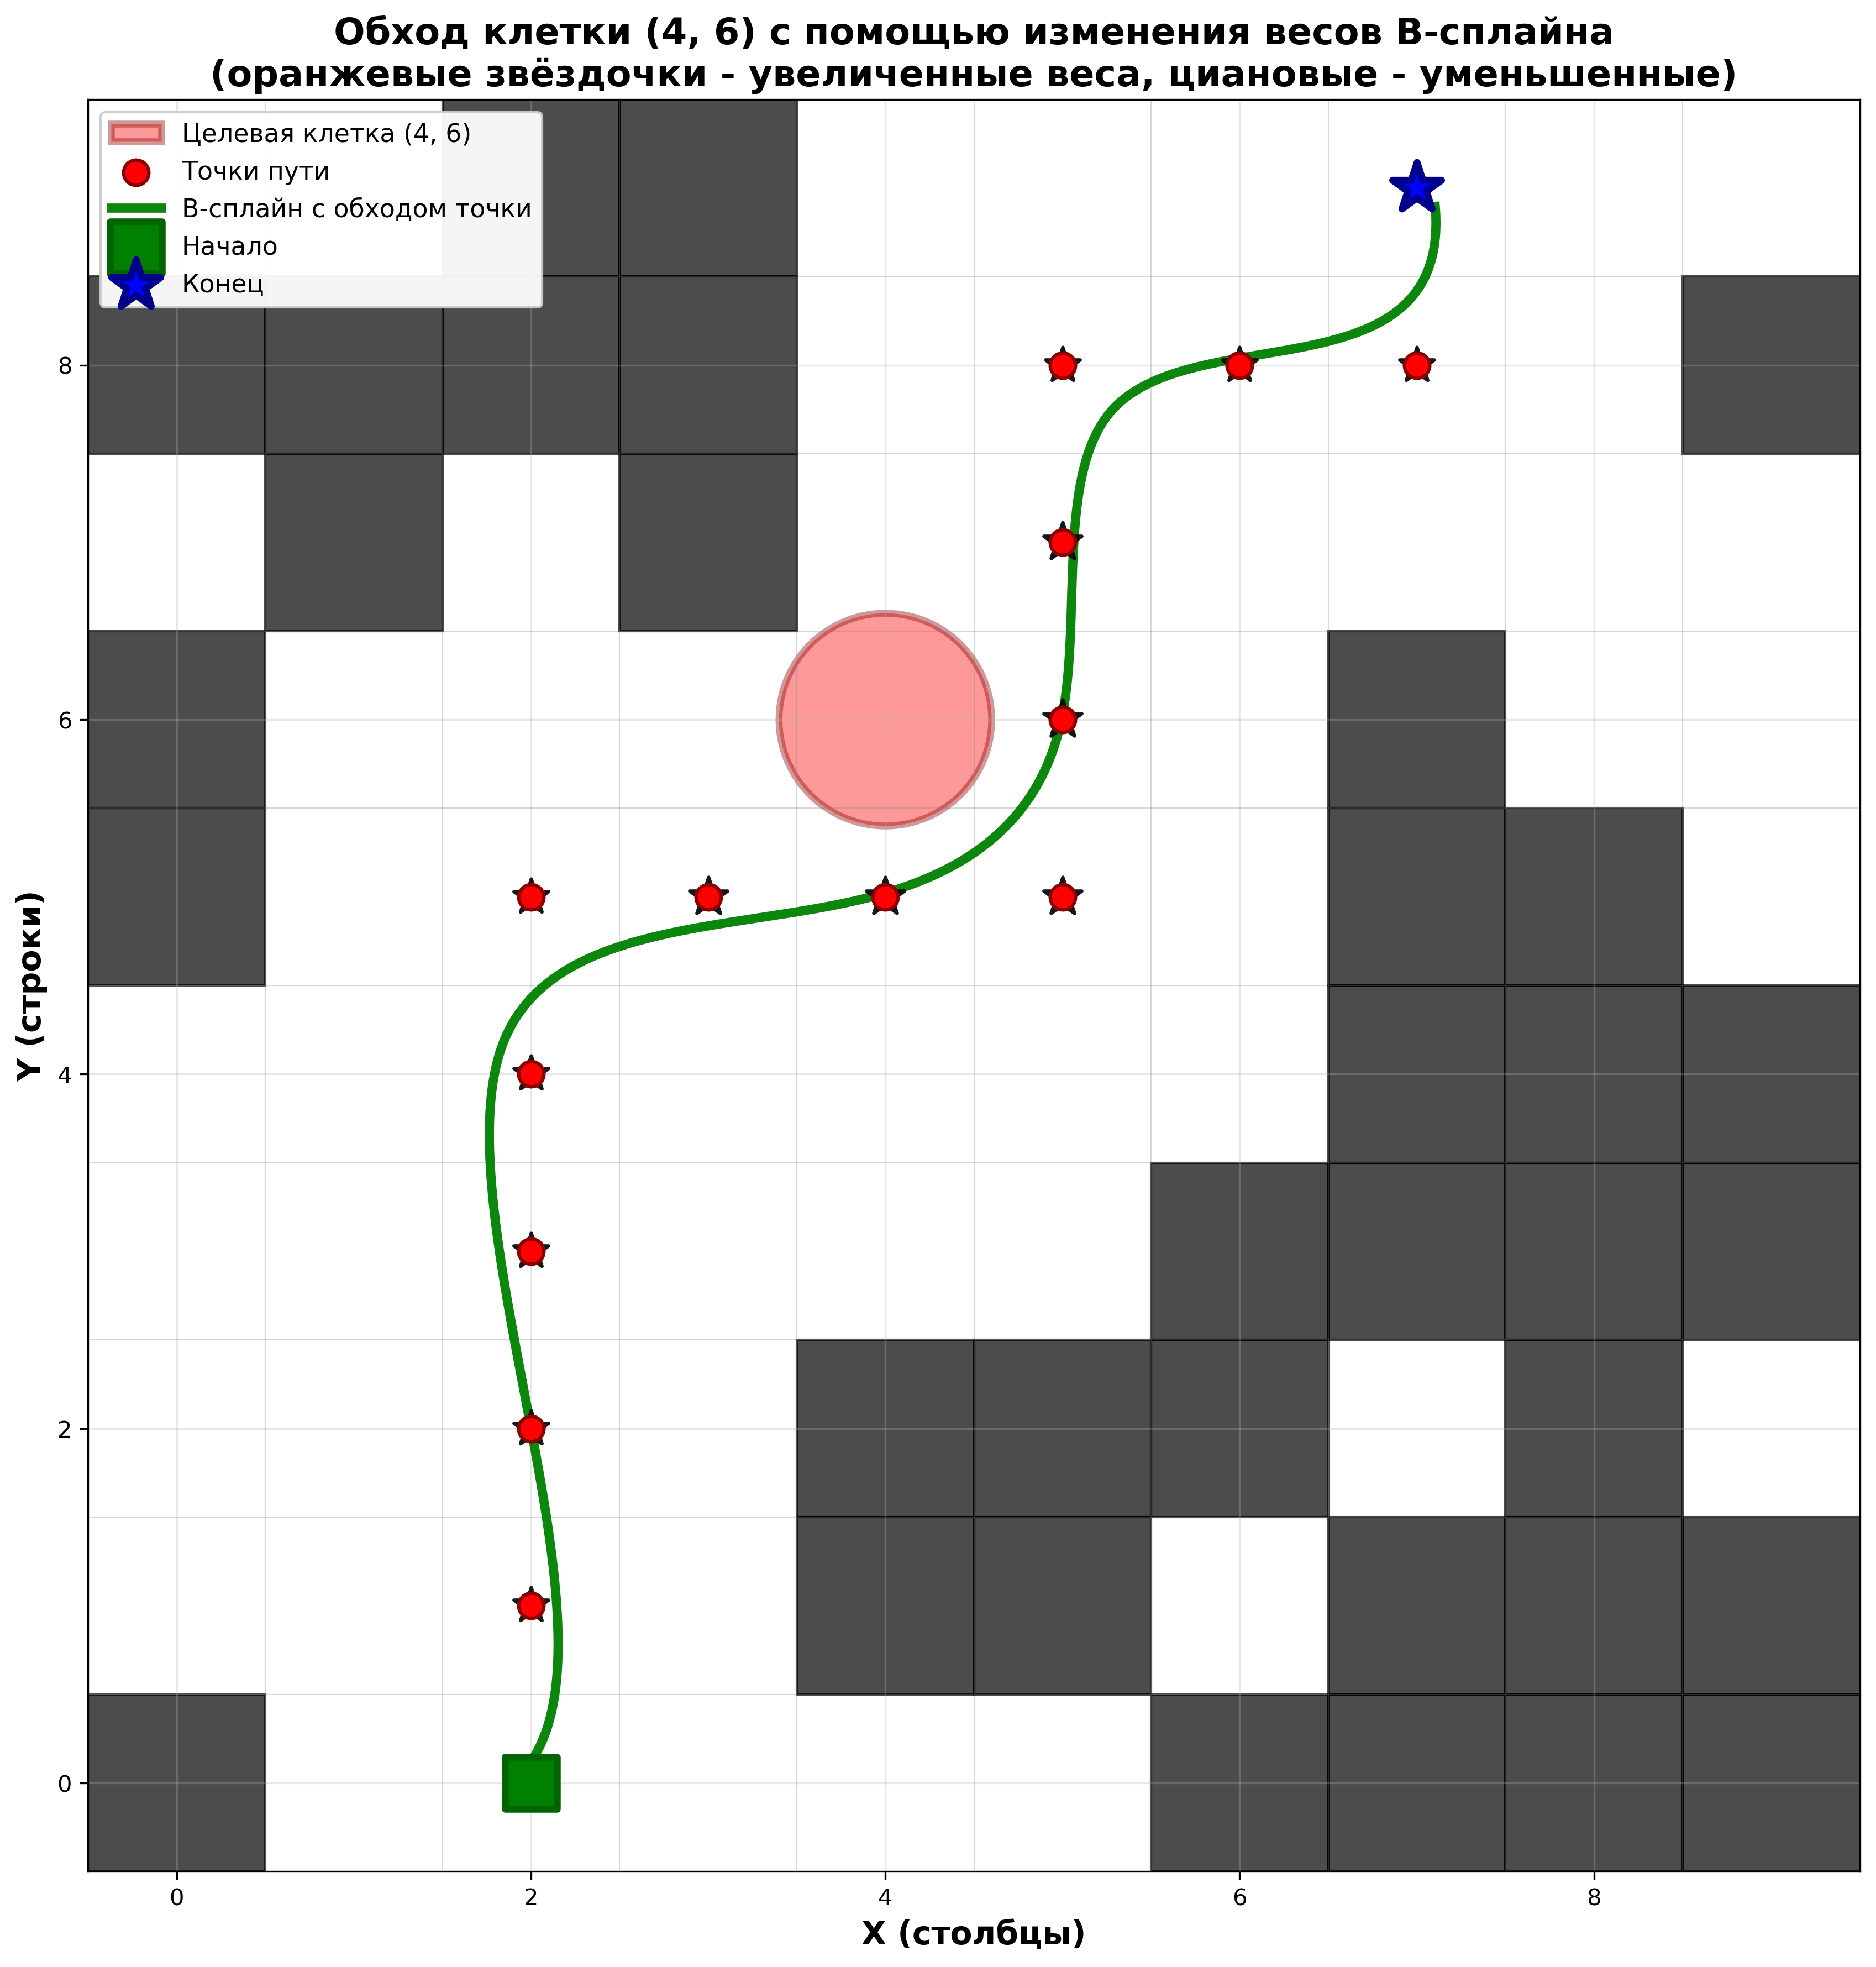
\includegraphics[width=0.9\textwidth]{images/task2/bspline_weighted_obstacle_avoidance.png}
\caption{B-сплайн траектория с обходом клетки (4, 6)}
\label{fig:weighted_bspline}
\end{figure}

Анализ полученной траектории показывает:
\begin{itemize}
\item Траектория успешно обходит целевую клетку (4, 6), проходя на безопасном расстоянии
\item Плавность и гладкость B-сплайна сохраняются
\item Минимальное отклонение от исходного пути, найденного алгоритмом A*
\item Визуально траектория не отличается от стандартного B-сплайна, сохраняя характерные плавные изгибы
\end{itemize}

\section{Выводы}

Изменение весов контрольных точек B-сплайна является эффективным методом для локальной адаптации траектории и обхода препятствий. Применение данного подхода позволяет:
\begin{itemize}
\item Обеспечить обход препятствия без существенного изменения формы траектории
\item Сохранить преимущества B-сплайнов (гладкость, локальный контроль)
\item Реализовать локальную модификацию траектории без пересчета всего пути
\end{itemize}

Предложенный метод может быть эффективно применен в задачах динамического планирования пути, где необходимо избегать внезапно появляющихся препятствий, не пересчитывая всю траекторию заново.

